
%(BEGIN_QUESTION)
% Copyright 2011, Tony R. Kuphaldt, released under the Creative Commons Attribution License (v 1.0)
% This means you may do almost anything with this work of mine, so long as you give me proper credit

In this process, maple syrup is heated as it passes through a steam heat exchanger, then enters an evaporator where the water boils off.  The purpose of this is to raise the sugar concentration of the syrup, making it suitable for use as a food topping.  A level control system (LT, LIC, and LV) maintains constant syrup level inside the evaporator, while an analytical control system (AT, AIR, AC, and AV) monitors the sugar concentration of the syrup and adjusts steam flow to the heat exchanger accordingly.

$$\includegraphics[width=15.5cm]{i03077x01.eps}$$

Suppose an operator notices the sugar concentration holding precisely to setpoint, and decides the controller need not be in automatic mode anymore.  After switching the AC to ``manual'' mode, the operator then leaves the controller to attend to other duties.  

\vskip 10pt

Describe in detail the effect this change in controller mode may (or will) have on the operation of this process.

\vskip 20pt \vbox{\hrule \hbox{\strut \vrule{} {\bf Suggestions for Socratic discussion} \vrule} \hrule}

\begin{itemize}
\item{} This is clearly {\it not} a recommended use of a controller's ``manual'' mode.  Describe at least one appropriate use of manual mode, and explain why manual mode is such a valuable feature in a process controller.
\end{itemize}

\underbar{file i03077}
%(END_QUESTION)





%(BEGIN_ANSWER)

%(END_ANSWER)





%(BEGIN_NOTES)

The syrup's sugar concentration will inevitably drift off setpoint as process loads vary.

\vskip 20pt \vbox{\hrule \hbox{\strut \vrule{} {\bf Virtual Troubleshooting} \vrule} \hrule}

This question is a good candidate for a ``Virtual Troubleshooting'' exercise.  Presenting the diagram to students, you first imagine in your own mind a particular fault in the system.  Then, you present one or more symptoms of that fault (something noticeable by an operator or other user of the system).  Students then propose various diagnostic tests to perform on this system to identify the nature and location of the fault, as though they were technicians trying to troubleshoot the problem.  Your job is to tell them what the result(s) would be for each of the proposed diagnostic tests, documenting those results where all the students can see.

During and after the exercise, it is good to ask students follow-up questions such as:

\begin{itemize}
\item{} What does the result of the last diagnostic test tell you about the fault?
\item{} Suppose the results of the last diagnostic test were different.  What then would that result tell you about the fault?
\item{} Is the last diagnostic test the best one we could do?
\item{} What would be the ideal order of tests, to diagnose the problem in as few steps as possible?
\end{itemize}


\vfil \eject

\noindent
{\bf Summary Quiz}

$$\includegraphics[width=15.5cm]{i03077x01.eps}$$

Suppose the steam tubes inside the heat exchanger gradually become coated (``fouled'') with residue from the raw maple syrup over time, making it more difficult (but not impossible) for adequate heat energy to transfer from the steam to the syrup.  Identify how this change will affect the process:

\begin{itemize}
\item{} The steam flow to the heat exchanger will be less than it was before the fouling
\vskip 5pt 
\item{} The steam valve (AV) will open up more than it was before the fouling
\vskip 5pt 
\item{} The level valve (LV) will pinch off (close) more than it was before the fouling 
\vskip 5pt 
\item{} The syrup entering the evaporator will be warmer than it was before the fouling
\vskip 5pt 
\item{} The syrup will exit the evaporator more concentrated than it was before the fouling
\vskip 5pt 
\item{} The level valve (LV) will open up more than it was before the fouling
\vskip 5pt 
\item{} The syrup will exit the evaporator less concentrated than it was before the fouling 
\end{itemize}

%INDEX% Basics, control loop troubleshooting: determining effect of specified fault(s)
%INDEX% Process: maple syrup concentration (single-effect evaporator)

%(END_NOTES)


